\startchapter{Literature Review}
\label{chapter:lit_review}

\newlength{\savedunitlength}
\setlength{\unitlength}{2em}

\section{Introduction}

Remote sensing is the acquisition of information about an object or phenomenon without the necessity of physical contact between it and the observer \cite{Gupta2018}. The human eyes, nose and ears are remote sensing instruments, collecting the electromagnetic, chemical and mechanical signals that comprise sight, smell and hearing, respectively.

In the geographic and earth sciences, remote sensing is typically (though not exclusively) conducted from above the earth using aircraft or space-borne satellites carrying instruments that measure electromagnetic or gravitational emissions from the Earth. Electromagnetic instruments may be further categorized as \emph{active}, such as LiDAR and RADAR which emit a pulse of radiation, then measure the temporal delay -- hence range -- of the echo, along with its intensity and other qualities; and \emph{passive}, which measure the reflected energy emitted by natural sources such as the sun or endogenous energy, such as thermal infrared radiation (i.e. heat).

Whatever instrument is used, distance from, and orientation relative to, the target has important impacts on the quality of information it produces, due to geometric (e.g., scale distortion or changes to the field of view), atmospheric (e.g. attenuation by scattering and absorption) and other effects. Changes in the instrument distance or orientation through time further impact the quality of data by inducing unpredictable variations in its characteristics: one cannot be confident, for example, that the statistical power of a result holds if the LiDAR point density from which it derives varies through space.

This research considers two types of remote sensing instruments typically used by UAV surveys: a ``pushbroom''-type hyperspectral imaging spectrometer (passive) and a scanning LiDAR device (active). 


\subsection{Imaging Spectroscopy}

%Electromagnetic energy -- photons -- may be detected using one of two types of detectors: photon detectors, in which photons free electrons from a substrate, generating an electrical current and thermal %detectors, which detect changes in their own temperature due to the absorption of light energy \cite{Wolfe1997}. These detectors can be characterized according to a set of objective quantities. The quantum %factor ($\eta$) is the ratio of electrons released to photons received, and is never greater than one. Responsivity is measured in volts (of output) per watt (of input), or a similar ratio. The quantum factor %tends to remain roughly constant across the detector's range of sensitivity, however, as photons at longer wavelengths are less energetic, the output voltage tends to drop significantly at the longer %wavelengths. Responsivity, meanwhile, usually increases linearly across the bandwidth of the element \cite{Wolfe1997}.

%Specific detectivity ($D*$) of a sensor is a figure of merit which gives an idea of the performance of a sensor, given its area, frequency bandwidth and noise characteristics. $D*$ is given by,

%\begin{equation}
%D* = \frac{\sqrt{A_d B}}{\Phi}SNR,
%\end{equation}

Goetz \emph{et al} \cite{Goetz1985} define hyperspectral imaging spectometry as ``the acquisition of images in many narrow contiguous spectral bands through the visible and solar-reflected infrared spectal bands simultaneously.'' Narrow spectral bands enable the detection of small absorbtion features which broad-band scanners, such as Landsat, cannot \cite{Goetz1985}. This is particularly important to researchers in agriculture, minerology and other fields where the discrimination of extremely narrow spectral features is necessary for the identification of physical features and phenomena \cite{Goetz1985}. 

Wolfe (\cite{Wolfe1997}) gives the specific detectivity ($D*$) of a spectrometer as,

\begin{equation}
D* = \frac{\sqrt{A_d B}}{\Phi}SNR,
\end{equation}

where $A_d$ is the detector area, $B$ is the effective noise bandwidth, $\Phi$ is the noise-equivalent power of the detector and $SNR$ is the signal to noise ratio. $D*$ is a figure of merit which gives an idea of the performance of a sensor, given its area, frequency bandwidth and noise characteristics. Unfortunately, decreasing the sensor area and narrowing the bandwidth (increasing spatial and spectral resolution, respectively) will increase the relative fraction of noise in the measurement \cite{Moses2012, Wolfe2997}.

The imaging spectrometers typically mounted on UAVs are of the linear-array ``pushbroom'' type, which have no moving parts and are therefore small and reliable enough for this purpose. In a pushbroom scanner, a single \emph{across-track}-aligned sensor array moves with the vehicle, with each sensor element receiving photons reflected from the target in a continuous swath parallel to the flight path. As the scanner moves across the target, the sensor measures and records radiant intensity (i.e. the number of reflected photons) in all bands during its \emph{integration time}. During the \emph{integration time}, all information captured by the element is saved as a single picture element, or pixel, which is spatially referenced to the target itself. 

The integration time of a scanner is related to another important quantity, \emph{dwell time}, by the platform velocity and field of view. Dwell time is the time during which a hypothetical object is recorded by the instrument. For a stationary instrument the dwell time and integration time are identical. For a moving instrument, dwell time may be equal to or less than the integration time and is contingent on platform velocity and altitude. For example, if an object at the forward edge of the detector at the beginning of the integration is at the rearward edge at the end of the integration, its dwell time is equal to the integration time. If an object were in the middle of the frame to begin with, its dwell time is half of the integration time. Raising the platform velocity would reduce both objects' dwell times with respect to the integration time, as they would cross the rearward edge of the pixel before recording ceased.


\subsubsection{Signal-to-Noise Ratio}

There are several sources of noise in hyperspectral imagery. 

\begin{itemize}
\item Shot noise \cite{Barducci2007} is due to the natural variability in the photon flux -- the number of photons passing through the sensor -- which follows a Poisson distribution;
\item thermal noise \cite{Barducci2007}, or dark current \cite{Rogass2011}, results from electrons generated spontaneously within the photosensitive material, as opposed to those activated by the interaction with a photon;
\item read noise \cite{Barducci2007} is produced during the generation of a charge from the instrument, and during analog-to-digital conversion;
\item charge transfer errors \cite{Barducci2007} result from defects in the sensor material;
\item round-off error \cite{Barducci2007}, or quantization error, which results when real numbers are rounded or truncated during conversion to a computer-representable form, and;
\item ``smearing'' \cite{Barducci2007,Ruyten1999}, which occurs as the photosensor remains active during charge transfer.
\end{itemize}

These sources have in common that they cannot not easily be mitigated by the user, but are intrinsic to the instrument. However, by increasing the magnitude of the signal, or photon flux, the relative influence of noise can be reduced \cite{Dor2012}. Of course, some of the factors affecting the strength of the signal cannot be directly controlled -- irradiant intensity, the properties of the instrument and the reflectivity of the target, to name a few -- but there are others that can:

\begin{enumerate}
\item A survey should be performed as near as possible to solar noon, the period of maximum irradiant intensity. 
\item The time interval during which photons are recorded by the instrument, the \emph{dwell time} \cite{Gupta2018,Goetz1985,Dor2012}, can be maximised. As the \emph{dwell time} increases, the contribution of background (additive) noise, relative to the signal and multiplicative noise, decreases. Thus \emph{dwell time} is critical to the maintenance of an acceptably high signal to noise ratio \cite{F.MarkDanson1996,Avery1992,Rogass2014}. Dwell time is a function of platform altitude, forward velocity and instrument field of view.
\item Increase the surface area of the target scanned during one integration. This is a function of platform altitude.
\item Minimize the thickness of the atmosphere between the instrument and target by minimizing the platform altitude.
\end{enumerate}

It is clear that items 2, 3 and 4 are in conflict and require careful consideration. It is also clear that while these issues can be optimized statically, they must be stabilized through time to guarantee the quality of collected data across the study area.

\cite{Gupta2018} gives a fundamental equation that relates various operating parameters of a sensor to signal-to-noise over a contiguous range of wavelengths as, 

\begin{equation}
\frac{S}{N} = \int_{\lambda_1}^{\lambda_2} \frac{ 
	I_{\lambda} \cdot T_{a(\lambda)} \cdot T_{o(\lambda)} \cdot \beta \cdot A_{O}D_{\lambda}^*
} {
	f \sqrt{\Delta f}
} \cdot d_{\lambda},
\end{equation}

where,

\begin{itemize}
\item $\lambda$ is the wavelength; 
\item $I_{\lambda}$ is the spectral radiance of the source as $\SI{} \watt \cm^{-2} sr^{-1} \micm^{-1} $; 
\item $T_{a(\lambda)}$ is the spectral transmittance of the atmosphere; 
\item $T_{o(\lambda)}$ is the spectral transmittance of the optical system; 
%\item $A_s$ -- the surface area of the target under view;
%\item $A_d$ -- the surface area of the detector;
\item $A_O$ is the effective area of the collector optic system; 
%\item $H$ -- the instrument-target distance;
\item $D_{\lambda}^*$ is the spectral detectivity of the sensor material; 
\item $d_{\lambda}$ is the \emph{dark current};
%\item $f$ -- the focal length of the optical system and ;
\item $\beta$ is the instantaneous field of view and;
\item $\Delta f$ is the electronic bandwidth, the speed with which electrons are carried away from the sensor.
\end{itemize} 

Here, $\beta$ can be further represented as, 

\begin{equation}
\beta_2 = \frac{A_s}{H_2},
\end{equation}

where, 

\begin{itemize}
\item $A_s$ is the surface area of the target under view and;
\item $H$ is the instrument-target distance.
\end{itemize}

It is clear that the signal-to-noise ratio, all other parameters held constant, is directly proportional to the platform height, as it effects the surface area of the target and thus the raw count of photons entering the instrument \cite{Gupta2018}. Though it is not possible to control the signal-to-noise ratio directly, it is possible to minimize it by careful selection of flight altitude, and to stabilize it by careful maintenance of the latter. For the purposes of this research, then, the goal is to treat the flight altitude as a proxy for signal-to-noise and to minimize the error between the planned trajectory altitude and the actual altitude.


%Most of the above inputs are intrinsic to the imaging system and are thus held constant, or to the target and light source which cannot be controlled, but $H$, $A_s$ and $T_{a(\lambda)}$ vary with the motion of the platform. This function can therefore be used to optimize the trajectory to minimize the variability of the signal-to-noise ratio. $A_s$ is also related to scale distortion, which can be minimized both \emph{along-track} with elevation and velocity, and \emph{across-track} with elevation and platform orientation. The $A_s$ term is related to the trade-off between spatial resolution and signal-to-noise ratio. Generally, the cell size and resolution are dictated by the survey specification so optimality implies minimizing the deviation from the specified spatial resolution, and minimizing the absolute signal-to-noise ratio, as well as its variability.

%It should be noted that this function does not separate out the contribubutions of atmospheric reflectance or specific sources of attenuation, nor does the present research require it. Calibration and correction are not within the scope of the project; rather, the goal is to minimize the variation in signal-to-noise ratio \emph{posterior} to the selection of an ideal survey altitude (in consideration of atmospheric effects), under the assumption that only the depth of the atmosphere (i.e. altitude) can be controlled.



%The total signal is given by the function,

%\begin{equation}
%S = \frac{\lambda}{hc} L_{\Delta \lambda} \frac{\pi}{4} \frac{ D^2}{f^2} p^2 T \eta_{sys},
%\end{equation}

%where,

%\begin{itemize}
%\item $\lambda$ -- the wavelength;
%\item $h$ -- Planck's constant;
%\item $c$ -- the speed of light ($\SI{}\m \s^{-1}$);
%\item $L_{\Delta \lambda}$ -- the incoming radiance in the waveband $\Delta \lambda$ ($\SI{} \watt \cm^{-2} sr^{-1} \micm^{-1} $);
%\item $D$ -- the diameter of the aperture ($\SI{}\m$);
%\item $f$ -- the focal length ($\SI{}\m$);
%\item $p$ -- the spatial width of a detector pixel ($\SI{}\m$);
%\item $T$ -- the exposure (integration) time ($\SI{}\s$);
%\item $\eta_{sys}$ -- the overall system efficiency.
%\end{itemize}

%[See \cite{Moses2012} for more about this]

\subsubsection{Geometric Distortion}

%[Tangent plane assumption of earth geometry -- ignore geodetic distortions]

\cite{Gupta2018} provides an extensive survey of the geometric causes of spectral image quality degradation. Geometric causes of degradation are grouped into two categories: systematic and non-systematic. Non-systematic distortions are due to variable or unpredictable factors such as airframe perturbation due to wind, while systematic distortions are those caused by fixed or planned effects, such as sensor-craft altitude and relief displacement.

Some variations in the velocity and attitude of the airframe and instruments are induced by forces (e.g. wind) which are stochastic in time and space and so not easily predicted. Others are induced by phenomena which are stochastic in space but constant in time and therefore predictable. Terrain relief is one of these. Variations in terrain relief induce changes in target distance for a platform and instrument travelling at a constant absolute elevation, which in turn induces geometric distortions in the imagery. Gupta \cite{Gupta2018} considers these disturbances to be non-systematic, but for the purposes of this research, they will be considered systematic and therefore addressable.

%[more]

\subsubsection*{Spectral Mixing}

As the target distance increases, with a constant IFOV, the surface area of the target captured in a single cell increases in proportion as, 

\begin{equation}
a\prime = a h^2,
\end{equation}

where $h$ is the platform altitude, $a$ is the target area and $a\prime$ is the final target area given a change in $h$. 

In a digital image, a cell, or pixel, has a constant area and a single value per band representing the measured radiance over the area contained within the spatial extent of the cell. A image, or raster, is a grid of cells. As a cell is the smallest unit that can be discriminated in a digital image, any objects within the cell will be impossible to isolate due to mixing. As the subject distance decreases, the target area within a cell decreases, enhancing the contribution of any individual object to the cell's overall value. At extremely high resolution, an object may fully occupy one or more cells. This is the essence of spatial resolution, and instrument and flight parameters are carefully chosen to optimize it to satisfy specific research objectives. 

An important consequence of spatial resolution is the phenomenon of ``spectral mixing'' whereby discrete objects within a pixel each contribute their spectra to an mixed spectrum within the pixel. Increasing the spatial resolution reduces aereal or linear mixing \cite{Gupta2018} while also increasing the signal-to-noise ratio: a cell, fully-occupied by an object of interest, is said to have a ``pure'' spectrum, which is considered to be desirable \cite{Gupta2018}. If a researcher is interested in the health of a particular plant, for example, she would not wish the reflected leaf spectra to be mixed with the spectra of soil or other objects. 

It is important that spectral mixing be held reasonably constant across the study area so that any results derived from the imagery can be considered to apply everywhere. ``Spectral unmixing'' is applicable as a post-processing step, but requires \emph{a priori} knowledge of the spectral signatures of the constituent objects in the scene, and the availability of a spectral library \cite{Adams1986,Smith1990,Gupta2018}.




~~~

 \cite{Gupta2018}. 
Quality in the geometric sense is determined by a series of identities relating to the characteristics of a sensor, its orientation, motion, distance from the target and the characteristics of the medium between the sensor and the target.

\cite{Avery1992}
Avery, T. E., \& Berlin, G. L. (1992). Fundamentals of Remote Sensing and Airphoto Interpretation (5th ed.).

Camera viewing angles.
Ground distance

~~~



\subsection{LiDAR}

Density - Statistical power, fractals, arc-curve.

Hypothesis testing, type I, II error, etc.

In \cite{DuPreez2014}, a method -- the arc-chord ratio (ACR) -- for estimating surface rugosity is given which takes the ratio of the surface area of a triangulated (i.e. Delaunay) point cloud and of the plane of best fit (POBF) of the boundary points of the cloud. Whereas the standard rugosity-estimation methods use the standard deviation or coefficient of variation of the point elevations, which stabilize as $n$ increases, the relationship of the ACR to point density is fixed, taking the form of an inverse parabola. The first derivative of the parabola at a given point density gives the fractal dimension at that point. In essence, increasing the point density decreases the size of the "ruler" used to measure the underlying structure.

Not only must $n$, or density, be sufficient to maintain the power of parametric statistical products, but the \emph{stability} of $n$ must be maintained in order to guarantee the quality of .... If the point counts are sufficient, either through low-altitude flying or large overlap, point density can be controlled artificially by removing a random selection of points from each cell. However, within a single flight line, an accurate altitude control system can fly the vehicle safely at a low enough elevation to maintain sufficient point density, while guaranteeing the consistency of the point density within certain bounds.



Overlap

\begin{figure} %[htbp] % htbp stand for "here", "top", "bottom", "page"
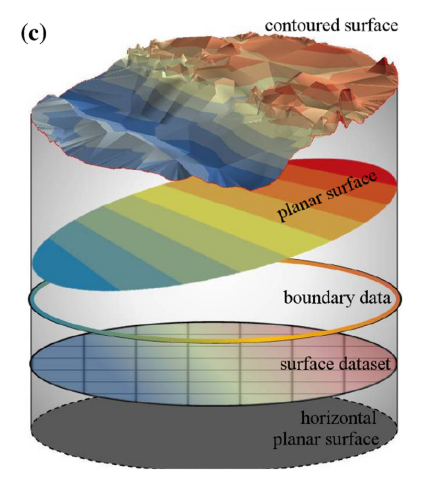
\includegraphics[scale=0.25]{tmp/dupreez_2014.pdf} 
\caption{Contoured surface and plane-of-best-fit used for arc-chord rugosity computation \cite{DuPreez2014}.}
\label{fig:arcchord}
\end{figure}


\subsubsection{Geometric Effects on Image Quality}


\section{Kinematics and Dynamics}

% The DJI API takes care of flight control, but a dynamical understanding of the platform is needed to set constraints on the optimization function.

% Quad/hex copter control inputs are highly coupled. It is not possible to rotate while horizontal McKerrow 2004

%The ideal trajectory would follow the terrain at a precise positive offset, but this is impossible for two reasons. First, if the terrain were to transition abruptly from one gradient to another, a discontinuity in the trajectory occurs, which, if the gradient increases, implies an infinite throttle input. This is obviously impossible, so the trajectory must be smoothed to such a degree that the vehicle's change in direction is achievable within the dynamical constraints on the vehicle, including the amount of available thrust. Second, it may not be desirable to follow the surface exactly, as navigating the vehicle into gaps between trees, for example, would be undesirable. In any case, the researcher has no interest in maintaining data quality between targets.



%The most directly addressable non-systematic (or semi-systematic) effect is caused by unwanted changes in platform orientation, specifically pitch. A multi-copter UAV moves horizontally by changing its thrust vector from vertical. Since the rotors are generally fixed to the airframe, the platform itself must assume a non-vertical pose during image acquisition. This is undesirable but unavoidable. However, in order to adjust its altitude or maintain horizontal velocity in the presence head- or tailwinds, the UAV may rotate further, causing geometric distortions in the imagery. 

%Mixing and Signal to Noise Ratio

%These distortions have two sources, first, the as the vehicle rotates forward on the y (\emph{across-track}) axis, the ground speed of the scanner footprint slows down. As the vehicle rotates to the rear, the footprint speeds up. This alters the \emph{dwell time} of the scanner and leads to over- and under-sampling, respectively \cite{Gupta2018}. When he vehicle rotates either to the fore or the rear, the scanner axis rotates away from nadir, increasing its effective footprint, inducing ``smear,'' reducing its spatial resolution \cite{Gupta2018} and increasing the effects of spectral mixing. 

%An important consequence of variation in \emph{dwell time} is the effect on the signal to noise ratio. The longer the \emph{dwell time}, the more light is measured by the instrument relative to the background noise \cite{Rogass2014}.

%An optimal trajectory would minimize these rotations, but in the attempt to minimize fore-aft platform rotation, it must be remembered that changes in velocity also affect \emph{dwell time}.


\subsubsection{Vehicle Dynamics and Control}

There are many aspects of vehicle dynamics that are unique to multi-rotor UAVs, some of which aid the stability of the vehicle. In particular, unlike a single-rotor helicopter, the rotors' torque forces cancel out, negating the need for a tail rotor, and the centre of mass is suspended between the rotors, rather than in line with the axis of rotation \cite{McKerrow2004}. A multi-copter is said to be an under-actuated system \cite{McKerrow2004,Mian2008,Valavanis2007} meaning that, though the vehicle has six degrees of freedom (rotation and translation along three axes), it has only four possible control inputs: roll, pitch, thrust and yaw. For this reason, it is virtually impossible for a human pilot to control a multi-copter directly, as one would a helicopter -- the advent of small, fast microprocessors, electro-mechanical control systems and sensors (e.g., gyroscopes and accelerometers) makes the entire field possible \cite{Hoffmann2007}. 


The goal of this research is not to design a complete multi-copter flight controller, but to use elements of control theory to send commands to the vehicle's flight control computer at the appropriate time. In particular, given the vehicle's mass, velocity, pitch, throttle position and altitude, when should the flight controller be instructed adjust the platform's elevation, and at what rate, in order to satisfy the error constraints, while not exceeding the flight envelope. For instance, if the flight controller is instructed too late to increase its altitude, it may diverge from the trajectory or it may collide with the terrain. Certainly, too large correction would entail the over-use of throttle and thus battery power.

In UAV remote sensing, the researcher will generally develop a flight plan that entails flying in a series of parallel lines within a study area polygon. As the vehicle approaches the end of each line, it crosses the boundary of the polygon, which functions as a "trigger box," stopping the instruments. The vehicle then turns, aligns on the next flight line and crosses back into the polygon, restarting the instruments. 

Since the horizontal control of the vehicle is handled by the mission-control software, this research will focus on the development of vertical trajectories only. There are then three control considerations: first, that the forward velocity of the platform is maintained; that the pitch of the vehicle is maintained; third, that the vertical trajectory is followed as closely as possible with the first two held as near constant as possible.

To satisfy the dual constraints of the flight envelope and the remote


~~~


The DJI Onboard Application Programming Interface (API) \cite{DJI2018} provides a means of retrieving various flight parameters from the flight computer at $\SI{100}\Hz$, including the hardware synchronization timestamp, the quaternion (orientation), angular rate, velocity and local and global positions. Combined with \emph{a-priori} knowledge about the mass, thrust and drag characteristics of the platform, this is enough information to determine the constraints upon the trajectory.


% \cite{MENON1991}'s formulation is attractive because it defines the vehicle's velocity vector in the tangent plane,
% orthogonal to the $z$-normal. The vehicle's velocity is in the $x$-$y$ plane, with respect to the ground surface as
% modelled, which preserves one of the constrains: constant ground velocity.


~~~

Part II Modelling and Control Fundamentals
Chapter 3: Airplane Basic Equations of Motion and Open-Loop Dynamics

Mostly dedicated to fixed-wing aircraft.
This is a superficial review, though still much beyond the scope of the current project (and way too mathy anyway).
Discussion of position and orientation of platform w/r/t frames (inertial, body, etc.), degrees of freedom, application of Newton’s laws.
Linear approximations of non-linear functions (aerodynamic forces, equations of motion, etc.) in order to make solutions tractable.
Body-fixed reference frame. C is the centre of mass, axis Cx is forward, Cz is down. Right-handed cartesian coordinate system.
Linear velocity components U, V, W, aligned with Cx, Cy and Cz.
Angular velocity components P, Q, R arounc Cx, Cy and Cz.
External aerodynamic forces X, Y, Z along axes. External aerodynamic moments as L, M, N.
Discussion of Euler angles for rotating the body frame relative to its fixed frame. (Twist around the z axis, rotate around y, rotate around z).
Important note that rotation order is important and not commutative.


This is a discussion of the relationships between the coordinate system of the platform and the inertial frame. There is a useful introduction to the way vector addition is used to calculate the displacement of objects relative to each other in three dimensions, and to the way that forces are calculated and transformed between frames. 
For this research, some basic kinematic equations are necessary for calculating the orientation of the rangefinder beam in real-time relative to the inertial frame (i.e. the Earth), given its position relative to the gimbal that creates the scan pattern, and the gimbal’s position relative the the platform and hence the inertial frame. 
The classical mechanics covered here will be necessary to calculate the forces acting on the platform in response to adjustments in the throttle to achieve an optimal (let alone possible) vertical trajectory, for calculating the thrust requirements and hence the power and power consumption.
Small Disturbance Theory - justification for the linearization of non-linear dynamic equations: when 

Chapter 4: Control Fundamentals of Small / Miniature Helicopters - A Survey

Discussion of the reduction in complexity of dynamic/control models to accommodate limited processing power. 
a) Attempt to model dynamics using parameters that represent physical forces; b) Use a reactive “black box” methodology where the parameters don’t model physical properties at all; c) Hybrid between a and b.
Assume “non-aggressive” flight, presumably to avoid control input singularities and exceeding the flight envelope.
Newton/Euler; Quaternions; Energy-oriented approach eg. the Lagrange formulation.

~~~

\cite{Kim2004}
Kim, S. K., \& Tilbury, D. M. (2004). Mathematical modeling and experimental identification of an unmanned helicopter robot with flybar dynamics. Journal of Robotic Systems, 21(3), 95–116. https://doi.org/10.1002/rob.20002

Helicopter kinematics using Euler angles. They justify their tolerance of singularities in this model because the vehicle will never point straight up or down. Singularity occurs at theta=+-pi/2
Position of vehicle w/r/t inertial frame defined by a position vector and Euler angles.
Velocities w/r/t inertial frame and body frame.
Rigid body equations - mass/inertia matrix.
Note: I think this project should ignore all aspects of vehicle dynamics except for symplified system which considers thrust, mass and inertia in order to create a simplified model of power over a trajectory. A model involving wind, etc. would be nice but let’s be serious here.


~~~

%\section{Computational Geometry}



\section{Trajectory Estimation}

[This is mostly over simple. The Menon journal article has a complete solution; also check the wiki for optimal control ]

see: Bianco2017


Since the objective of this research is to derive a trajectory which optimises certain constraints, it must be representable by a function. In general, it is desireable for the trajectory to be smooth and twice-differentiable to eliminate singularities in the control inputs, for example, the need for infinite thrust to satisfy the demand for an infinite rate of climb, or an instantaneous change in said rate \cite{MENON1991,Funk1977}. 

Much of the work on trajectory estimation has been conducted for the military into the automated control of ballistic missiles \cite{Dressler1968}, helicopters and fixed-wing aircraft \cite{MENON1991,Funk1977}. In a military context, aside from physical constraints, there is a need for ``terrain masking'' -- evading radar and other forms of detection by hiding the aircraft behind terrain features. This requires that the aircraft follow the terrain at a low, roughly constant altitude, putting extraordinary demands on the control system and airframe \cite{MENON1991}. Fortunately, the requirements of military aircraft dovetail nicely with those of remote-sensing aircraft.

All authors define the objective in terms of a simple function. \cite{MENON1991} uses, 

\begin{equation}
F(x,y) = h_c + f(x,y) + P(x,y)
\end{equation}

where $F(x,y)$ gives the trajectory elevation at the given downrange ($x$) and crossrange ($y$), and $h_c$ is the altitude with respect to the terrain, either constant or as a function. Other constraints, such as, in the military context, ``threats'' and obstacles to the vehicle, are modelled by $P(x,y)$. Ultimately, the result is a smoothed model of the terrain with some minimal offset corresponding to the desired elevation.

\cite{MENON1991} and \cite{Funk1977} suggest the use of cubic spline interpolation to produce twice-differentiable curves suitable for trajectory estimation, while \cite{Funk1977} suggests building the operational constraints into the spline equation. This allows the definition of a maximum curvature of the trajectory in respect of the craft's flight envelope. Piecewise splines are ideal for this application as, so long as the slope and elevation are identical where they meet, continuity is insured.

\cite{Funk1977} provides several key concepts that relate by analogy to the demands of UAV remote sensing. The ``frame length'' concept concerns the distance required to execute a ``characteristic manouvre'' \cite{Funk1977} -- a ``symmetric manouvre'' over an obstacle of ``maximum expected height'' (typically three times rugosity -- the standard deviation in the terrain elevation), including maximum pull-up, push-over and transition arcs. The symmetric manouvre is represented using piecewise cubic splines whose integrals must sum to zero for the resumption of level flight. In the fixed-wing military aircraft context, the constraints are those imposed by flight envelope of the craft. A remote-sensing UAV is no different, however, rather than airframe integrity, lift and thrust (etc.), the constraints on a UAV primarily concern the availability of thrust and rotational velocity (for thrust vectoring), as well as whatever bounds are placed data-quality and power consumption.

Through ``efficient programming'' for the CDC 6600 computer, Funk proposes a $\SI{3}{\second}$ frame time which, at Mach 1, would yield a trajectory update every $\SI{1067}{\m}$ \cite{Funk1977}. For a relatively high (for a UAV) horizontal velocity of $\SI{10}{\m\/\s}$, this gives an update every $\SI{30}{\m}$. Given the advances in computer technology in the intervening 41 years -- the CDC 6600 was introduced in 1967 and weighed $\SI{5400}{\tonne}$ -- $\SI{3}{\second}$ would be an extremely pessimistic estimate for a trajectory update period using presently-available hardware.

There have been other methods for deriving trajectories, but these have drawbacks that render them unsuitable for remote-sensing UAV applications. Twigg, Calise and Johnson (\cite{Twigg2003}) extend Menon's (\cite{MENON1991}) work through the notion of constant-energy, rather than constant-velocity trajectory estimation, however the maintenance of a constant ground speed is critical to the data-quality objectives of this research.


Per The use of a spline curve trajectory that incorporates the given constraints has the advantage of modelling said constraints while decoupling the flight control inputs from trajectory estimation. *


~~~

Unmanned underwater vehicles
Artificial Neural Networks
Sensors pointed fore and aft, and one pointed down.

Though there is relatively little research on the present problem -- predictive trajectory estimation based on forward-looking terrain modeling for UAV applications -- there is plenty of research on terrain avoidance for both autonomous underwater vehicles (AUVs) and ballistic missiles, as far back as the 1950s. 
AUVs
[Maybe note that underwater vehicles are a good path for study because they are larger and can carry a lot of hardware, have military significance and support, etc]

\cite{Samar2011}
Samar, R., \& Rehman, A. (2011). Autonomous terrain-following for unmanned air vehicles. Mechatronics, 21(5), 844–860. https://doi.org/10.1016/j.mechatronics.2010.09.010

Requires a pre-generated DEM
To develop a “reference trajectory in the vertical plane” that the vehicle will follow, within the constraints of the flight envelope.
Constraints on climb and descent rate [n.b. Impacts battery consumption, data quality]
Definition of trajectory error w/r/t terrain elevation.
Discusses INS drift and the role this plays in extracting accurate elevation data from DEM -- “corridor of uncertainty.”
Max elevation within a circle of uncertainty is used as the reference elevation.
Two algorithms, “Stair Algorithm” and “Spline Algorithm”.
Stair algorithm goes some way to solving the ‘valley’ problem, where a gap in surface is encountered that we don’t want to go into.
Cubic splines.
“The spline trajectory is smooth as expected and is optimal in the sense of minimizing the objective function.”
“Convergence issues” with spline.
Quality index: “the integral over range of the difference between the actual terrain and the trajectory generated by the algorithm, i.e., R edR (note that e is constrained to be positive semidefinite). “
Stair algorithm produces instantaneous changes in trajectory which:
Result in large throttle inputs (battery wasteage, etc.)
Failure to track (overshooting the corners on descent)
Tracking controller design - plant model.
Flight control hardware, software, testing, etc.

\cite{Twigg2003}
Twigg, S., Calise, A., \& Johnson, E. (2003). On-Line Trajectory Optimization for Autonomous Air Vehicles. In AIAA Guidance, Navigation, and Control Conference and Exhibit (pp. 1–9). Reston, Virigina: American Institute of Aeronautics and Astronautics. https://doi.org/10.2514/6.2003-5522

Constant-energy vs. constant velocity constraint for vertical trajectory.
Lagrangian and Hamiltonian stuff

\cite{Waldock1995}
Waldock, M. I. (1995). Terrain following control of an unmanned underwater vehicle using artificial neural networks. In IEE Colloquium on `Control and Guidance of Remotely Operated Vehicles’ (Vol. 1995, pp. 4–4). IEE. https://doi.org/10.1049/ic:19950800

\cite{Bovio2006}
Bovio, E., Cecchi, D., \& Baralli, F. (2006). Autonomous underwater vehicles for scientific and naval operations. Annual Reviews in Control, 30(2), 117–130. https://doi.org/10.1016/j.arcontrol.2006.08.003

Military AUVs - control system requirements: course-keeping, constant depth, constant altitude, noise and disturbance rejection. All relevant to UAVs.
Rejection of high-frequency noise (that is, terrain variations) in this case due, for example, to plants -- Poseidonia oceanica -- Mediterranean sea grass, leaves up to 1.5m long.
Model-dependent vs. model-independent control systems -- the former depend on accurate modeling of the physical parameters of the platform and are subject to changes. The latter is robust to platform changes but more complex to implement [or was at the time this was published…]
Control loop:

Suggest INS for best navigation system.
Kalman filter error estimation.
Instrumentation:
IMU
Speed sensor (doppler velocity log)
Depth/pressure
Independent position sensor (GPS) for initialization and error resets.

\cite{Jalving1994}
Jalving, B. (1994). The NDRE-AUV Flight Control System. IEEE Journal of Oceanic Engineering, 19(4), 497–501. https://doi.org/10.1109/48.338385

AUV using PID control with equations, etc.
Used for constant elevation (not terrain following)

NO CITE
A.J. Healey, \& Lienard, D. (1993). Multivariable sliding mode control for autonomous diving and steering of unmanned underwater vehicles. Oceanic Engineering, IEEE Journal Of, 18(3), 327–339. https://doi.org/10.1109/JOE.1993.236372

Sliding mode control, dynamic equations, etc.

\cite{Juul1994}
Juul, D. L., Mcdermott, M. E., Nelson, E. L., Barnett, D. M., \& Williams, G. N. (1994). Submersible Control Using the Linear uadratic Gaussian with Loop Transfer ecovery Metha.

\cite{FeijunSong}
Feijun Song, \& Smith, S. M. (n.d.). Design of sliding mode fuzzy controllers for an autonomous underwater vehicle without system model. OCEANS 2000 MTS/IEEE Conference and Exhibition. Conference Proceedings (Cat. No.00CH37158), 2, 835–840. https://doi.org/10.1109/OCEANS.2000.881362

\cite{Goheen1990}
Goheen, K. R., \& Jefferys, E. R. (1990). Multivariable Self-Tuning Autopilots for Autonomous and Remotely Operated Underwater Vehicles. IEEE Journal of Oceanic Engineering, 15(3), 144–151. https://doi.org/10.1109/48.107142

\section{Surface Reconstruction}

Geometric vs. statistical surface reconstruction

Berger, M., Tagliasacchi, A., Seversky, L. M., Alliez, P., Guennebaud, G., Levine, J. A., … Silva, C. T. (2017). A Survey of Surface Reconstruction from Point Clouds. Computer Graphics Forum, 36(1), 301–329. https://doi.org/10.1111/cgf.12802

Priors - the assumptions that one uses to focus the reconstruction of the surface:
“Our survey presents surface reconstruction algorithms from the perspective of priors: assumptions made by algorithms in order to combat imperfections in the point cloud and to eventually focus what information about the shape is reconstructed. Without prior assumptions, the reconstruction problem is ill-posed; an infinite number of surfaces can pass through (or near) a given set of data points”
Some priors involve low-level data characteristics. Some involve higher-level structural factors.
Constrain expectations, prioritize desireables
Eg. Dense, uniform point cloud -> smoothness prior
Studies a variety of reconstruction methods, priors and issues. 
Fairly technical.


One aspect of the surface reconstruction that must be considered is the shape of the surface, which requires an exploration of the notion of shape. The convex hull is one such notion of shape. There are a variety of sufficient descriptions, one being that it is the set that encloses all segments joining each point in the point cloud to each other point. For any given point set, there is exactly one convex hull.

Edelsbrunner and Müke \cite{Edelsbrunner1994}	provide a similarly rigorous definition of shape, using $\alpha$-shapes. The $\alpha$-shape is a generalization of the convex hull, which is best understood using the ice cream metaphor \cite{cgal:dy-as3-18b}. If one imagines the point cloud as a collection of chocolate chips embedded in ice cream, one can scoop out the ice cream between the chips, leaving behind a shape. The remaining shape is determined by the squared radius ($\alpha$) of the scoop. An $\alpha = \inf$ scoop (a plane) will leave the convex hull itself, while a $\alpha = 0$ scoop will leave only the chocolate chips. So, for any given $\alpha$ there is exactly one solution, but $\alpha$ itself is bounded by $[0-\inf]$.

The $\alpha$-shape reconstruction my be valuable for this case as it offers a parameter that satisfies the requirement that pits or holes in the terrain of a certain size may be closed or filled in. Plus, the algorithm is usually implemented using the Delaunay triangulation, which can be computed incrementally on a point stream.
\section{Control Systems}

%There are two primary fields of control system development, model-based and reactive. Model-based systems attempt to re-create the physical forces and control inputs acting upon a vehicle in order to calculate the control inputs required to maintain a stable state. Reactive controls, on the other hand, use sensor inputs to determine the amount of error between the desired and actual states, and compute the control inputs required to reduce the error.

\subsubsection{PID Controllers}

[discuss actuator saturation and control input singularity for hard-angled trajectories, etc.]


The \emph{proportional-integral-derivative} controller (PID) is widely used in industry \cite{Soediono1989} to maintain the stability of, for example, chemical processes by measuring process outputs, calculating the error with regards to a target metric and feeding the measurements back into the controller which adjusts the input actuators. This paradigm has the advantage that it doesn’t necessarily require a comprehensive physical model of the process to succeed, only a desired outcome and the possibility of achieving that outcome by adjusting the available inputs (a closed-loop system) \cite{Soediono1989}. PID controllers are often self-training and can be considered a form of primitive artificial intelligence.

PID controllers are ideally suited to the complex state-management tasks that face a multi-rotor UAV. In fact, controlling such an inherently-unstable vehicle would be nearly impossible without the assistance of some sort of automated controller. It is not always possible, given changing payloads, environmental conditions, terrains and flight plans -- not to mention the availability of comprehensive models and computing power -- to accurately model a vehicle’s dynamics ahead of time. 

PID control originated early in the 20th century when it was found that the work of properly managing the stability of industrial manufacturing processes was too difficult for an individual worker \cite{Bennett2001}. Numerous firms and individuals worked on the development of pneumatic linear-feedback systems which used the flapper nozzle mechanism as a kind of gain amplifier, which could sense changes in a system and actuate a response. It was not until 1939 that a true PID emerged.

Per \cite{Soediono1989}, the PID control law consists of the sum of three control actions:

\begin{itemize}
\item The proportional action $K_p$ is proportional to the control error as, 

\begin{equation}
u(t) = K_p e(t) = K_p(r(t) - y(t)),
\end{equation}

where $u$ is the output, or controlled variable and $e$ is the control error (the difference between the reference signal and the output signal). 

\item The integral action $K_i$ relates to integral gain, 

\begin{equation}
u(t) = K_i \int_0^t e(\tau) d\tau,
\end{equation}

or the sum of errors over time. 

\item The derivative action $K_d$, 

\begin{equation}
u(t) = K_d \frac{de(t)}{dt},
\end{equation}

relates to the slope of trend in error over time.
\end{itemize}

The proportional term can be understood as the current error state; the integral term is over the sum of past states and the derivative term is a prediction of future states \cite{Soediono1989}. The control system is then the sum of the three terms, 

\begin{equation}
u(t) = K_p + K_i + K_d,
\end{equation}




General PID for Industrial Processes:
\cite{Saxena}
Chidambaram, M., \& Saxena, N. (2018). Relay Tuning of PID Controllers. Singapore: Springer Singapore. https://doi.org/10.1007/978-981-10-7727-2

Ref’ed: Handbook of PI and  PID controller tuning rules; PID control in the third millennium; Practical PID control
Plenty of different loop tuning methods.

\cite{Sanchez2012}
Sánchez, J., Visioli, A., \& Dormido, S. (2012). PID Control in the third millenium. PID Control in the Third Millennium. https://doi.org/10.1007/978-1-4471-2425-2

\cite{Soediono1989}
Soediono, B., \& Visioli, A. (2006). Practical PID Control. (Intergovernmental Panel on Climate Change, Ed.), Climate Change 2013 - The Physical Science Basis (Vol. 53). Cambridge: Springer London. https://doi.org/10.1007/1-84628-586-0

\section{Operating Systems}

A typical modern desktop computer divides its tasks into units of work which it dispatches to the processor to be performed. This is called multitasking. All current mainstream operating systems (OSX, Windows and Linux) use a strategy called preemptive multitasking, whereby a currently-executing process may be preempted by another process if the first process is, for example, waiting on a resource, or has a lower priority than the new process. On a single core, no two processes execute at the same time, but interleaving operations gives the impression of simultaneous execution and can radically speed up execution of a set of tasks if one or more of those tasks is required to wait for any reason. Task scheduling is performed by the scheduler according to one a variety of heuristics.

Multitasking computers used for flight-control and other time-critical operations have one or more processes that must not be preempted, lest a critical operation fail to complete in sufficient time to keep the craft safely aloft. A multitasking operating system that permits non-preemptable threads of execution is called a realtime operating system (RTOS) \cite{Foundation2018,BristotdeOliveira2018}. Realtime operating systems allow processes to execute without interruption and require those processes to complete within a specified temporal bound \cite{BristotdeOliveira2018}. Failure to meet a deadline results in system failure. Ultimately, the goal of the RTOS is to provide deterministic bounds on the execution times of tasks \cite{BristotdeOliveira2018}.

The Linux operating system three realtime scheduling policies in the standard kernel, \texttt{SCHED\_FIFO}, \texttt{SCHED\_RR} and \texttt{SCHED\_DEADLINE} \cite{Foundation2018,BristotdeOliveira2018}. \texttt{SCHED\_FIFO} and \texttt{SCHED\_RR} use the POSIX scheduler and are similar in that they require a thread to run to completion, unless a thread with a higher priority preempts it. Under \texttt{SCHED\_FIFO} (first-in-first-out), tasks are executed at in the order in which they arrive, while \texttt{SCHED\_RR} executes tasks in sequential order using a circular queue. 

\texttt{SCHED\_DEADLINE} uses the deadline scheduler. Each task is configured with a run time, a deadline and a period. For deadline-scheduled tasks, the run time is guaranteed to be available within each period, and the task will complete before the deadline \cite{BristotdeOliveira2018}. Linux' deadline scheduler uses the 	Global Earliest Deadline First (GEDF) algorithm which schedules tasks with the earliest deadlines first. On multi-core systems this can cause tasks to miss their deadlines, even when processor utilization is blow maximum. For example, if four tasks with short deadlines are assigned to each of four cores, a single long-running task will be unable to complete before its deadline (the Dhall effect). Alternatively, if the four short tasks were assigned to run in sequence on one core, the long-running task could complete on another, leaving two cores free \cite{BristotdeOliveira2018a}. In multi-core environments, it is therefore necessary to run critical tasks on a CPU  reserved for that purpose, leaving other tasks to run on the remaining CPUS.

Typically, kernel tasks are not preemptible. That is, only threads in ``user space'' can be suspended while a higher-priority task executes. The \texttt{PREEMPT\_RT} patch adds two preemption modes to the kernel, Preemptible Kernel (Basic RT) and Fully Preemptible Kernel (RT). With the fully preemptable kernel selected, all kernel code is preemptible, save for certain highly critical sections which are reduced through alternative locking constructs  \cite{Foundation2018}. The \texttt{PREEMPT\_RT} patch can be applied to any Linux kernel, including that used by the Raspbian distribution used by Raspberry Pi.

\section{Ethics}

Clearly, a project that seeks to wrest control from an autonomous aerial platform, with the potiential to harm humans and animals and damage property, must justifiable on ethical grounds. The ``Handbook of Unmanned Aerial Vehicles'' \cite{Valavanis2015j} contains several chapters by different authors on the subject of ethics and autonomous, or semi-autonomous, machines. These are discussed mostly in the context of warfare, using the ethical frameworks developed by scholars of war.

The chapter, ``Ethics and UAVs'' \cite{Valavanis2015bz} begins by addressing the employment of UAVs as weapons. (In this context, UAVs are often pejoratively called ``drones'', to distinguish them from more neutral scientific uses, though the names given to these machines -- ``Predator,'' ``Reaper'' and ``Crusher'' \cite{Lucas2011} -- leave little doubt as to their purpose.) So long as UAVs continue to be controlled, remotely, by a human operator, the ethical landscape remains more-or-less unchanged, versus more hands-on methods of waging war, with several exceptions relating to the feasibility of missions that would not be otherwise possible if an on-site human operator were required. This includes targeted assasinations, which entail the risk of mis-identifying civilians as targets (a possible war crime) and of conducting missions in regions which are not theaters of war. In addition, the accessibility of this technology enables non-state actors (private companies, individuals and militias) to engage in remote warfare \cite[p.2867]{Valavanis2015bz}. 

The inevitable advent of total autonomy muddies the water further: when a machine commits what would otherwise be considered a war crime, who is accountable? Lucas calls this proposition ``preposterous'', arguing that machines are incapable of forming intentions and are therefore incapable of committing crimes \cite[p.2868]{Valavanis2015bz}. This criticism seems to beg the question, however, as a human being \emph{is} a sort of machine and is clearly capable of having intention. Less controversially, perhaps, humans also routinely invest their prejudices into the machines they build \cite{Greenwald1998,Caliskan2017}. 

The chapter becomes a philosophical digressesion into the ethics of autonomous machines but resolves with a meditation on the ethical responsibility of engineers \cite[p.2873]{Valavanis2015bz} revolving around Michael Waltzer's notion of ``double intention'' \cite{Waltzer}. Under this rubric, originally intended to articulate the ethical responsibilities of soldiers, an engineer has the duty not only to \emph{intend} to do no harm, but to exercise \emph{due care} \cite{Lucas2011} -- to take all reasonable steps necessary to ensure that no harm occurs. The chapter ends with an admonishment to engineers to become aware of and center their ethical responsibilities \cite[p.2974]{Valavanis2015bz}.


\setlength{\unitlength}{\savedunitlength}
